\documentclass[../TDO1-O2.tex]{subfiles}%

\begin{document}
\section[s]"2"{Rayon lumineux à travers une vitre}
\enonce{%
	Un rayon lumineux traverse une vitre d'épaisseur $a = \SI{5.0}{mm}$ et d'indice
	$n = \num{1.5}$ sous une incidence $i_1 = \ang{45;;}$. Le milieu extérieur est
	l'air.
}%

\QR{%
	Faire un schéma et calculer l'angle de réfraction $i_2$ lors du
	passage à travers la première face (air$\rightarrow$verre). Calculer
	alors l'angle de réfraction $i_3$ lors du passage à travers la
	deuxième face (verre$\rightarrow$air).
}{%
	\begin{tcbraster}[raster columns=11, raster equal height=rows]
		\begin{tcolorbox}[blankest, raster multicolumn=5, space to=\myspace]
			\begin{tcbraster}[raster columns=1]
				\begin{tcn}[raster multicolumn=1](data){Schéma}
					\begin{center}
						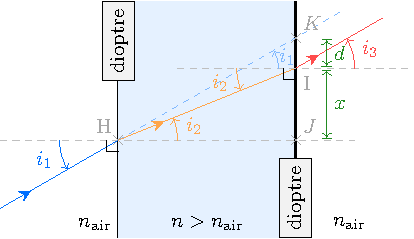
\includegraphics{vitre}
					\end{center}
				\end{tcn}
				\begin{tcn}[add to natural height=\myspace](tool){Outils}
					Loi de \textsc{Snell-Descartes}:
					\[n_1\sin i_1 = n_2\sin i_2\]
				\end{tcn}
			\end{tcbraster}
		\end{tcolorbox}
		\begin{tcolorbox}[blankest, raster multicolumn=6, space to=\myspace]
			\begin{tcbraster}[raster columns=1]
				\begin{tcn}[raster multicolumn=1](ques)'r'{Résultat attendu}
					Le rayon passe deux dioptres de l'air au verre, puis du verre à l'air.
					On utilise \textsc{Snell-Descartes} pour déterminer la direction du
					rayon émergent et la comparer à celle du rayon incident.
				\end{tcn}
				\begin{tcn}[sidebyside, righthand width=1.5cm,
						add to natural height=\myspace](appl)'r'{Application}
					\begin{itemize}[leftmargin=40pt]
						\olditem[\textbf{En H}] : $\sin i_1 = n\sin i_2$\smallbreak
						\hspace{-40pt}$\Leftrightarrow
							i_2 = \arcsin(\sin(i_1)/n) = \ang{28;;}$;
						\olditem[\textbf{Dedans}] : $i_2$ aux deux dioptres ;
						\olditem[\textbf{En I}] : $\sin i_3 = n\sin i_2$ ;
						\olditem[\textbf{D'où}] :
						$\cancel{n_1}\sin i_3 = \cancel{n_1}\sin i_1$
					\end{itemize}
					\tcblower
					Ainsi,
					\[\boxed{i_3 = i_1}\]
					(retour inverse)
				\end{tcn}
			\end{tcbraster}
		\end{tcolorbox}
	\end{tcbraster}
}%
\QR{%
	Justifier que le rayon entrant et le rayon sortant sont parallèles.
}{%
	Comme les dioptres sont parallèles, leurs normales le sont aussi.
	Ainsi, les rayons émergent et incident sont parallèles.
}%

\QR{%
	Calculer la déviation latérale $d$ (la distance entre le point où sort
	le rayon émergeant et celui où sortirait le rayon incident s'il n'était
	pas dévié) entre ces deux rayons.
}{%

	$\DS\tan(i_2) = \frac{\rm IJ}{\rm HJ} = \frac{x}{a}$ et $\DS\tan(i_1) =
		\frac{x+d}{a}$, d'où $\DS\frac{d}{a} = \tan(i_1) - \frac{x}{a} =
		\tan(i_1) - \tan(i_2)$, soit
	\[
		\boxed{d = a(\tan(i_1) - \tan(i_2))}
		\quad\text{avec}\quad
		\left\{
		\begin{array}{rcl}
			a   & = & \SI{5.0}{mm} \\
			i_1 & = & \ang{45;;}   \\
			i_2 & = & \ang{28;;}
		\end{array}
		\right.\]
	C'est-à-dire
	\[
		\boxed{d = \SI{2.3}{mm}}
	\]
}%

\end{document}
